\chapter{Theory and Motivation}

The Standard Model (SM) of particle physics is our current best theory to describe the fundamental particles and their interactions.
The SM describes the strong force, as well as unifying the weak and electromagnetic forces.
The latter is partly done through the Brout-Englert-Higgs (BEH) mechanism for spontaneous symmetry breaking, that allows many fundamental particles to obtain masses.
It also predicts a new scalar boson, named the Higgs boson.
In 2012, the ATLAS \cite{ATLAS_Higgs_Discovery} and CMS collaboration \cite{CMS_Higgs_Discovery} discovered a Higgs boson-like particle when colliding protons at high energy at the Large Hadron Collider (LHC) and further measurements of this particle's properties have been consistent with such a particle.
This discovery experimentally completed the SM particle constituents. \\

However, the SM is not without theoretical problems and experimental tensions.
Firstly, the hierarchy problem describes the issue of lightness of the observed Higgs boson mass and the "unnatural" balancing of inputs needed to explain the theorised loop corrections to the predicted mass. 
These are orders of magnitude larger than then observed mass.
A solution to this problem is Supersymmetry, but no experimental evidence for this theory has yet been found that separates it from the Standard Model. 
Secondly, results from the LHCb experiment \cite{} and the g−2 experiment \cite{} have shown deviations from the SM predictions.
Although not the statistical significance for a discovery, they offer intriguing hints at potential Beyond SM (BSM) physics.
BSM particles, produced from extended Higgs sectors or otherwise, have been theorised to explain these deviations .
This chapter will explain the SM and the Higgs sector theory, as well as detailing the BSM extensions that can help resolve the theoretical tensions and experimental tensions.

\section{The Standard Model of Particle Physics}

\subsection{Fundamental Particles and Interactions}

The SM is a set of fundamental particles, as shown in Figure~\ref{fig:sm_diagram}, and rules that govern the interactions between particles.
The interactions between these particles are able to model the strong, weak and electromagnetic force, unifying the later two into one electroweak interaction.
The SM consists of 6 quarks, 3 charged leptons and 3 neutrinos, which are named fermions. 
Each of these particles contain an anti-partner with opposite quantum numbers but the same mass.

The SM is a renormalisable quantum field theory that is built on the principle of local gauge invariance.
The SU(3) $\otimes$ SU(2) $\otimes$ U(1) is the gauge symmetry group of the SM.
This means that the Lagrangian, that governs the particles interactions, is invariant under such a transformation.

\begin{figure}[!hbtp]
\centering
    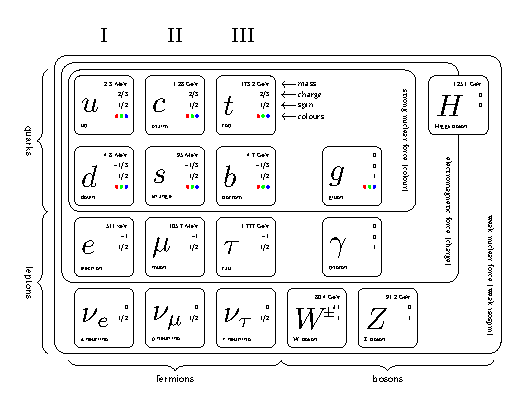
\includegraphics[width=\textwidth]{Figures/SM_diagram.pdf}
\caption{}
\label{fig:sm_diagram}
\end{figure}

\subsection{Higgs Sector}

\begin{equation}
	\Phi = 
	\begin{pmatrix} 
		\phi^{+} \\
		\phi^{0} \\
	\end{pmatrix}
\end{equation}

\begin{equation}
	\mathcal{L} = (\partial_{\mu}\phi)^{\dagger} (\partial^{\mu}\phi) - V(\phi)
\end{equation}

\begin{equation}
V(\phi) = \mu^2 \phi^{\dagger} \phi + \lambda (\phi^{\dagger} \phi)^2
\end{equation}

Has minima at
\begin{equation}
\phi^{\dagger} \phi = -\frac{\mu^2}{2\lambda}
\end{equation}

Need massless photon
\begin{equation}
\braket{0|\phi|0} = \frac{1}{\sqrt{2}}
	\begin{pmatrix} 
		0 \\
		\nu \\
	\end{pmatrix}
\end{equation}

Break symmetry

\begin{equation}
\phi = \frac{1}{\sqrt{2}}
	\begin{pmatrix} 
		0 \\
		\nu + h(x)\\
	\end{pmatrix}
\end{equation}

To make the mass term gauge invariant

\begin{equation}
\partial_{\mu} \rightarrow D_{\mu} = \partial_{\mu} + \frac{i g_{W}}{2} \vec{\sigma} \cdot \vec{W}_{\mu} + \frac{ig^{'}Y}{2} B_{\mu}
\end{equation}

\begin{equation}
D_{\mu}\phi =  \frac{1}{\sqrt{2}}
	\begin{pmatrix} 
		0 \\
		\nu + h(x)\\
	\end{pmatrix}
\end{equation}

\section{Extended Higgs Sector}

There is no theoretical limitation to only have one Higgs doublet in the theory.
Therefore, a natural extension to the SM Higgs sector is the two Higgs doublet model (2HDM).

\begin{equation}
\begin{aligned}
\mathcal{L}^{\text{2HDM}}_{\text{yukawa}} &= - \sum_{f=u,d,l}\Big(\frac{m_{f}}{\nu}g^{f}_{h}\bar{f}fh + \frac{m_{f}}{\nu}g^{f}_{H}\bar{f}fH -i\frac{m_{f}}{\nu}g^{f}_{A}\bar{f}\gamma_{5}fA\Big)  \\ 
&- \Big[\frac{\sqrt{2}V_{ud}}{\nu}\bar{u}(m_{u}g^{u}_{A}P_{L} + m_{d}g^{d}_{A}P_{R})dH^{+} + \frac{\sqrt{2}m_{l}g^{d}_{A}}{\nu}\bar{\nu}_{L}l_{R}H^{+} + h.c.\Big]
\end{aligned}
\end{equation}

\begin{table}[H]
    \centering
    \begin{tabular}{|x{1.0cm}|x{2.0cm}x{2.0cm}x{2.0cm}x{2.0cm}|}
    		\hline
    	 	& Type I & Type II & Type X & Type Y \\
    	 	\hline
    	 	\hline
    	 	$u$ & $\Phi_2$ & $\Phi_2$  & $\Phi_2$  & $\Phi_2$  \\ 
    	 	$d$ & $\Phi_2$ & $\Phi_1$ & $\Phi_2$ & $\Phi_1$ \\
    	 	$l$ & $\Phi_2$ & $\Phi_1$   & $\Phi_1$    & $\Phi_2$ \\
        \hline
    \end{tabular}
    \caption{}
\end{table}

\begin{table}[H]
    \centering
    \begin{tabular}{|x{1.0cm}|x{2.0cm}x{2.0cm}x{2.0cm}x{2.0cm}|}
    		\hline
    	 	& Type I & Type II & Type X & Type Y \\
    	 	\hline
    	 	\hline
    	 	$g_{h}^{u}$ & $c_{\alpha}/s_{\beta}$ & $c_{\alpha}/s_{\beta}$  & $c_{\alpha}/s_{\beta}$  & $c_{\alpha}/s_{\beta}$  \\ 
    	 	$g_{h}^{d}$ & $c_{\alpha}/s_{\beta}$ & $-s_{\alpha}/c_{\beta}$ & $c_{\alpha}/s_{\beta}$  & $-s_{\alpha}/c_{\beta}$ \\
    	 	$g_{h}^{l}$ & $c_{\alpha}/s_{\beta}$ & $-s_{\alpha}/c_{\beta}$ & $-s_{\alpha}/c_{\beta}$ & $c_{\alpha}/s_{\beta}$  \\
    	 	\hline
    	 	$g_{H}^{u}$ & $s_{\alpha}/s_{\beta}$ & $s_{\alpha}/s_{\beta}$ & $s_{\alpha}/s_{\beta}$ & $s_{\alpha}/s_{\beta}$ \\
    	 	$g_{H}^{d}$ & $s_{\alpha}/s_{\beta}$ & $c_{\alpha}/c_{\beta}$ & $s_{\alpha}/s_{\beta}$ & $c_{\alpha}/c_{\beta}$ \\
    	 	$g_{H}^{l}$ & $s_{\alpha}/s_{\beta}$ & $c_{\alpha}/c_{\beta}$ & $c_{\alpha}/c_{\beta}$ & $s_{\alpha}/s_{\beta}$ \\
    	 	\hline
    	 	$g_{A}^{u}$ & $1/t_{\beta}$ & $1/t_{\beta}$ & $1/t_{\beta}$  & $1/t_{\beta}$ \\
    	 	$g_{A}^{d}$ & $1/t_{\beta}$ & $t_{\beta}$   & $-1/t_{\beta}$ & $t_{\beta}$ \\
    	 	$g_{A}^{l}$ & $1/t_{\beta}$ & $t_{\beta}$   & $t_{\beta}$    & $-1/t_{\beta}$ \\
        \hline
    \end{tabular}
    \caption{}
\end{table}

\section{Theoretical Problems and Potential Solutions}

\subsection{Hierarchy Problem}

\begin{figure}[H]
\centering
    \begin{subfigure}[b]{0.4\textwidth}
    \centering
    \scalebox{0.8}{
    \begin{tikzpicture}
    \begin{feynman}
    \vertex (a) {\(H\)};
    \vertex [right = 1.5cm of a] (b);
    \vertex [right = 1cm of b] (dummy);
    \vertex [right = 1cm of dummy] (c);
    \vertex [above = 1cm of dummy] (e);
    \vertex [below = 1cm of dummy] (f);
    \vertex [right = 1.5cm of c] (d) {\(H\)};
    \diagram* {
    (a) -- [scalar] (b),
    (b) -- [out=90, in=180] (e),
    (e) -- [out=0, in=90, edge label=\(f\)] (c),
    (b) -- [out=-90, in=180] (f),
    (f) -- [out=0, in=-90] (c),
    (c) -- [scalar] (d)
    };
    \end{feynman}
    \end{tikzpicture}
    }
    \caption{}
    \label{fig:corr_fermion}
    \end{subfigure}
    \begin{subfigure}[b]{0.4\textwidth}
    \centering
    \scalebox{0.8}{
    \begin{tikzpicture}
    \begin{feynman}
    \vertex (a) {\(H\)};
    \vertex [right = 2cm of a] (b);
    \vertex [right = 2cm of b] (c) {\(H\)};
    \vertex [above = 1cm of b] (dummy);
    \vertex [left = 1cm of dummy] (d);
    \vertex [above = 1cm of dummy] (e);
    \vertex [right = 1cm of dummy] (f);
    \diagram* {
    (a) -- [scalar] (b),
    (b) -- [scalar, out=180, in=-90] (d),
    (d) -- [scalar, out=90, in=-180] (e),
    (e) -- [scalar, out=0, in=90, edge label=S] (f),
    (f) -- [scalar, out=-90, in=0] (b),
    (b) -- [scalar] (c)
    };
    \end{feynman}
    \end{tikzpicture}
    }
    \caption{}
    \label{fig:corr_scalar}
    \end{subfigure}
    \caption{One-loop corrections to the Higgs mass by a fermion f (a) and a scalar S (b).}
    \label{fig:Higgs_One_Loop_Corrections}
\end{figure}

The hierarchy problem can be resolved by adding a symmetry between fermions and bosons that allow cancellations to corrections to the Higgs mass. This theory is known as Supersymmetry. \cite{SUSY_Primer} In its simplest form, the Minimal Supersymmetric Standard Model (MSSM), is a type-II 2 Higgs doublet model (2HDM), the predicts the existence of five Higgs bosons: two scalars (h, H), two charged bosons (\(H^{\pm}\)) and one pseudoscalar (A). At tree level this Higgs sector only depends on two parameters, $m_A$ and $\tan\beta$, where $\tan\beta$ is the ratio of vacuum expectation values.

\begin{equation}
\tan \beta = \frac{\langle H_{u}^{0} \rangle}{\langle H_{d}^{0} \rangle} = \frac{v_{u}}{v_{d}}
\end{equation}

The couplings of the neutral Higgs bosons to heavy fermions are different from the Standard Model Higgs couplings. At tree level these differ by the factors shown in the Table \ref{tab:mssm_couplings}.


Due to the hierarchy of the top and bottom masses, it is expected that $\tan\beta$ is greater than 1 and therefore the couplings to tau leptons and bottom quarks would be enhanced and the coupling to top quarks would be suppressed.

Eq.(\ref{eqn:dm_f}) and Eq.(\ref{eqn:dm_S}) show that if the mass of the scalar is equivalent to that of the fermion and \(\lambda_f = \lambda_{S}^{2}\), then the Higgs mass corrections cancel. This offers a solution to the hierarchy problem introducing a new symmetry that extends the Standard Model. The symmetry relates fermions and bosons and is known as Supersymmetry. It states that fermions and bosons exist in groups called supermultiplets. Each supermultiplet contains fermion and boson states which are superpartners of one another. On-shell each supermultiplet must have an equivalent number of fermionic and bosonic degrees of freedom. In order for this to also hold off-shell, an auxiliary field is added to balance the number of degrees of freedom. Extending this theory to currently known particles, the simplest set of supermultiplets can be found and are shown in Tables \ref{tab:MSSM_Chiral} and \ref{tab:MSSM_vector}. \\

Two Higgs supermultiplets are needed due to the anomaly cancellation condition, Tr[\(T_{3}^{2}Y\)] = Tr[\(Y^3\)] = 0, where \(Y\) and \(T_3\) are the third components of weak hypercharge and isospin respectively. The Higgs chiral supermultiplet, the higgsino, makes a significant contribution to the trace as it has a weak hypercharge \(Y=+\frac{1}{2}\). This anomaly is solved by introducing another Higgs chiral supermultiplet, with a higgsino of weak hypercharge \(Y=-\frac{1}{2}\), so that the traces cancel. This results in five physical Higgs boson states. 

\begin{table}[H]
\centering
\begin{tabular}{c||ccc}
     \hline
     Names & Spin \(\frac{1}{2}\) & Spin 1 & \(SU(3)_C, SU(2)_L, U(1)_Y \)\\
     \hline
     \hline
     Gluino, gluon & \(\tilde{g}\) & \(g\) & \((\textbf{8},\textbf{1},0)\) \\
     Winos, W bosons & \(\tilde{W}^{\pm}\) \(\tilde{W}^{0}\) & \(W^{\pm}\) \(W^0\) & \((\textbf{1},\textbf{3},0)\) \\
     Bino, B boson & \(\tilde{B}^{0}\) & \(B^0\) & \((\textbf{1},\textbf{1},0)\) \\
     \hline
\end{tabular}
\caption{The Minimal Supersymmetry Standard Model Vector Supermultiplets \cite{SUSY_Primer}.}
\label{tab:MSSM_vector}
\end{table}


The \(Z^{0}\) and \(\gamma\) states are found by mixing the \(W^0\) and \(B^0\) states after electroweak symmetry breaking in the Standard Model. There corresponding gauginos that are named zino (\(\tilde{Z}^0\)) and photino (\(\tilde{\gamma}\)) are found by the same method from the \(\tilde{W}^0\) and \(\tilde{B}^0\). \\

If Supersymmetry is an unbroken theory, then one would expect to have the superpartners at the same mass as the Standard Model particles. This has not been seen experimentally, therefore Supersymmetry must be a broken theory in the vacuum state. One can define soft supersymmetry breaking through the addition of SUSY violating Lagrangian term \(\mathcal{L}_{\text{soft}}\), where

\begin{equation}
    \mathcal{L} = \mathcal{L}_{\text{SUSY}} + \mathcal{L}_{\text{soft}}.
\end{equation}

\(\mathcal{L}_{\text{soft}}\) contains only mass terms and coupling parameters. Defining \(m_{\text{soft}}\) as the largest mass scale involved in the soft Lagrangian, \(m_{\text{soft}}\) also then defines the mass splitting between the Standard Model particles and the sparticles. If the mass splitting becomes significant, the hierarchy problem would be reintroduced as corrections to the Higgs mass would again become large.

The MSSM Higgs sector is CP-conserving at tree level. It contains a light, \(h\), and a heavy, \(H\), CP-even Higgs boson, a CP-odd Higgs boson, \(A\), and two charged Higgs bosons \(H^{\pm}\). The parameters of the sector can all be obtained from three factors: the Z boson mass, \(m_Z\), the CP-odd Higgs mass, \(m_A\), and \(\tan\beta\), where

\begin{equation}
    \tan \beta = \frac{\langle H_{u}^{0} \rangle}{\langle H_{d}^{0} \rangle} = \frac{v_u}{v_d}.
\end{equation}

\(\tan \beta\) is the ratio of the vacuum expectation values of the neutral components of the Higgs doublets. The masses of the \(h\), \(H\) and \(H^{\pm}\) Higgs bosons at tree level are calculated to be \cite{mssm_theory}

\begin{subequations}
\begin{align}
    m_{\text{h}}^2 = & \frac{1}{2}\Big(m_{\text{A}}^2 + m_{\text{Z}}^2 - \sqrt{(m_{\text{A}}^2 + m_{\text{Z}}^2)^2 - 4 m_{\text{Z}}^2 m_{\text{A}}^2 \cos^2{2\beta}} \Big), \\
    m_{\text{H}}^2 = & \frac{1}{2}\Big(m_{\text{A}}^2 + m_{\text{Z}}^2 + \sqrt{(m_{\text{A}}^2 + m_{\text{Z}}^2)^2 - 4 m_{\text{Z}}^2 m_{\text{A}}^2 \cos^2{2\beta}} \Big), \\
    m_{\text{H}^{\pm}}^2 = & m_{\text{A}}^2 + m_{\text{W}}^2.
\end{align}
\end{subequations}

All of the tree level couplings can also be expressed in terms of these three parameters but they will not all be stated here. The main couplings of interest for this report are that between the neutral Higgs bosons and heavy fermions. These couplings are the largest of the Higgs sector. The couplings of the three heaviest fermions to the MSSM Higgs sector are shown in the below Table \ref{tab:MSSM_coupling}. \\

Due to the mass hierarchy of the top and bottom quarks, it is expected that \(\tan\beta\) lies in the range

\begin{equation}
    1 \lesssim \tan\beta \lesssim \frac{m_t}{m_b}.
\end{equation}


\section{Experimental Tensions and Potential Solutions}

\subsection{B Anomalies}

Recent measurements from the LHCb experiment, testing lepton flavour conservation, have found deviations away from the Standard Model. The measurement of $R_{K}$, $R_{K^{*}}$ and $R_{D(^{})}$ have deviations with significances of 3.1, 2.1-2.5 and 3.1 $\sigma$ respectively \cite{Rk,Rkstar,Rd}. These B-anomalies have prompted the idea for a short range lepton flavour violating interaction. This interaction is theorised to be mediated by leptoquarks. In an attempt to fit a model that offers a combined explanation of these results, it was found that a $U_{1}$ vector leptoquark was the only leptoquark that could offer a simultaneous explanation of all anomalous results \cite{leptoquark}. Such a leptoquark would couple to fermions by the Lagrangian shown below.

\begin{equation}
\lag_{U} = \frac{g_{U}}{\sqrt{2}} U^{\mu} \big[ \beta_{L}^{i\alpha}( \bar{q}_{L}^{i} \gamma_{\mu} l_{L}^{\alpha}) + \beta_{R}^{i\alpha}( \bar{d}_{R}^{i} \gamma_{\mu} e_{R}^{\alpha}) \big] + \text{h.c.}
\end{equation}

where $g_{U}$ is the coupling scaling parameter and $\beta_{L}$ and $\beta_{R}$ are the left and right-handed mixing matrices

\begin{equation}
\beta_{L} = 
\begin{pmatrix}
0 & 0 & \beta_{L}^{d\tau} \\
0 & \beta_{L}^{s\mu} & \beta_{L}^{s\tau} \\
0 & \beta_{L}^{b\mu} & 1
\end{pmatrix},
\hspace{1cm}
\beta_{R} = 
\begin{pmatrix}
0 & 0 & 0 \\
0 & 0 & 0 \\
0 & 0 & \beta_{R}^{b\tau}
\end{pmatrix}.
\end{equation}

The fit to B-anomolies done in Ref. \cite{leptoquark}, found the best fit values for each left-handed mixing matrix parameter based on two scenarios for $\beta^{b\tau}_{R}$, namely $\beta^{b\tau}_{R} = 0$ and $\beta^{b\tau}_{R} = -1$. These represents no and maximal right-handed contributions. The most stringent constraints on these models are imposed by high-$p_{T}$ di-tau tails. At the LHC the most dominant production mode of this final state would be given in Figure \ref{fig:leptoquark_feynman}.

\subsection{g-2 Anomaly}

In the alignment limit, for the normal scenario $h_{SM}=h$, $sin(\beta-\alpha)=1$, $\implies$ $c_{\alpha}/s_{\beta}=1$, $s_{\alpha}/c_{\beta}=-1$, $s_{\alpha}/s_{\beta}=-1/t_{\beta}$, $c_{\alpha}/c_{\beta}=t_{\beta}$.

In the alignment limit, for the inverted scenario $h_{SM}=H$, $cos(\beta-\alpha)=1$ $\implies$ $c_{\alpha}/s_{\beta}=1/t_{\beta}$, $s_{\alpha}/c_{\beta}=t_{\beta}$, $s_{\alpha}/s_{\beta}=1$, $c_{\alpha}/c_{\beta}=1$.


\begin{table}[H]
    \centering
    \begin{tabular}{p{1.5cm}|x{2.2cm}x{2.2cm}x{2.2cm}x{2.2cm}}
         \hline
         Scenario & $\tan\beta$ & $m_{A}$ (GeV) & $m_{\phi}$ (GeV) & $m_{H^{\pm}}$ (GeV) \\
         \hline
         \hline
         Normal & $\geq 90$ & [62.5,145] & [130,245] & [95,285] \\
         Inverted & $\geq 120$ & [70,105] & [100,120] & [95,185] \\
         \hline
    \end{tabular}
    \caption{}
    \label{tab:gm2region}
\end{table}